%% 
%% Copyright 2007-2019 Elsevier Ltd
%% 
%% This file is part of the 'Elsarticle Bundle'.
%% ---------------------------------------------
%% 
%% It may be distributed under the conditions of the LaTeX Project Public
%% License, either version 1.2 of this license or (at your option) any
%% later version.  The latest version of this license is in
%%    http://www.latex-project.org/lppl.txt
%% and version 1.2 or later is part of all distributions of LaTeX
%% version 1999/12/01 or later.
%% 
%% The list of all files belonging to the 'Elsarticle Bundle' is
%% given in the file `manifest.txt'.
%% 
%% Template article for Elsevier's document class `elsarticle'
%% with harvard style bibliographic references

%%\documentclass[preprint,12pt,authoryear]{elsarticle}

%% Use the option review to obtain double line spacing
%% \documentclass[authoryear,preprint,review,12pt]{elsarticle}

%% Use the options 1p,twocolumn; 3p; 3p,twocolumn; 5p; or 5p,twocolumn
%% for a journal layout:
%% \documentclass[final,1p,times,authoryear]{elsarticle}
%% \documentclass[final,1p,times,twocolumn,authoryear]{elsarticle}
%% \documentclass[final,3p,times,authoryear]{elsarticle}
%% \documentclass[final,3p,times,twocolumn,authoryear]{elsarticle}
%% \documentclass[final,5p,times,authoryear]{elsarticle}
\documentclass[final,5p,times,twocolumn,authoryear]{elsarticle}

%% For including figures, graphicx.sty has been loaded in
%% elsarticle.cls. If you prefer to use the old commands
%% please give \usepackage{epsfig}

%% The amssymb package provides various useful mathematical symbols
\usepackage{minted}
\usepackage{amssymb}
\usepackage{amsmath}
%% The amsthm package provides extended theorem environments
%% \usepackage{amsthm}
\usepackage{aas_macros}
\usepackage{fontawesome}
%% The lineno packages adds line numbers. Start line numbering with
%% \begin{linenumbers}, end it with \end{linenumbers}. Or switch it on
%% for the whole article with \linenumbers.
%% \usepackage{lineno}

\usepackage{xcolor}
\definecolor{xlinkcolor}{cmyk}{1,1,0,0}
\usepackage[colorlinks = true,
            linkcolor = xlinkcolor,
            urlcolor  = xlinkcolor,
            citecolor = xlinkcolor,
            anchorcolor = xlinkcolor]{hyperref}

\newcommand{\nblink}[1]{\href{https://github.com/DifferentiableUniverseInitiative/jax-cosmo-paper/blob/master/notebooks/#1.ipynb}{\faFileCodeO}}
\newcommand{\github}{\href{https://github.com/DifferentiableUniverseInitiative/jax\_cosmo}{\faGithub}}



\journal{Astronomy and Computing}


%%%% new command (JEC)
\newcommand{\nn}{\nonumber}
\newcommand{\numpyro}{\texttt{NumPyro}}
\newcommand{\bydef}{:=}


\begin{document}

\begin{frontmatter}

%% Title, authors and addresses

%% use the tnoteref command within \title for footnotes;
%% use the tnotetext command for theassociated footnote;
%% use the fnref command within \author or \address for footnotes;
%% use the fntext command for theassociated footnote;
%% use the corref command within \author for corresponding author footnotes;
%% use the cortext command for theassociated footnote;
%% use the ead command for the email address,
%% and the form \ead[url] for the home page:
%% \title{Title\tnoteref{label1}}
%% \tnotetext[label1]{}
%% \author{Name\corref{cor1}\fnref{label2}}
%% \ead{email address}
%% \ead[url]{home page}
%% \fntext[label2]{}
%% \cortext[cor1]{}
%% \address{Address\fnref{label3}}
%% \fntext[label3]{}

\title{jax-cosmo: End-to-End Differentiable and GPU Accelerated Cosmology Library}

%% use optional labels to link authors explicitly to addresses:
%% \author[label1,label2]{}
%% \address[label1]{}
%% \address[label2]{}

\author{jax-cosmo contributors}

\address{}

\begin{abstract}
With jax-cosmo, Fisher forecasts are accurate and instantaneous, inference is lightning-fast, survey optimization is trivial. \github
\end{abstract}

%%Graphical abstract
%\begin{graphicalabstract}
%\includegraphics{grabs}
%\end{graphicalabstract}

%%Research highlights
%\begin{highlights}
%\item Research highlight 1
%\item Research highlight 2
%\end{highlights}

\begin{keyword}
%% keywords here, in the form: keyword \sep keyword

%% PACS codes here, in the form: \PACS code \sep code

%% MSC codes here, in the form: \MSC code \sep code
%% or \MSC[2008] code \sep code (2000 is the default)

\end{keyword}

\end{frontmatter}

%% \linenumbers

%% main text

\section{Introduction}
Monte Carlo Markov Chain Bayesian inference is a widely used technique in Cosmology since the work of \citep{2001ApJ...563L..95K,2003MNRAS.341.1084R} and has been the keystone for CMB analysis thanks to software as  \texttt{CosmoMC}\footnote{\url{https://cosmologist.info/cosmomc/readme.html}} \citep{2002PhRvD..66j3511L} as well as   \texttt{Cobaya}\footnote{\url{https://cobaya.readthedocs.io}} \citep{2019ascl.soft10019T,2021JCAP...05..057T} which is the baseline option for the current on going cosmological experiments.

Although these package does not take benefit of recent advance in automatic differentiation (aka \textit{autodiff}) \citep{2015arXiv150205767G, 2018arXiv181105031M} which is been widely used in neural network optimization and more generally for machine learning and computational statistics as for instance Hamiltonian Monte Carlo sampling and Variational Inference, two subjects covered in this paper. The \textit{autodiff} has been implemented in widely used libraries as for instance \texttt{Stan}\footnote{\url{https://mc-stan.org/users/documentation}} \citep{JSSv076i01} and \texttt{TensorFlow}\footnote{\url{https://www.tensorflow.org/}}  \citep{tensorflow2015-whitepaper}. 

Recently, the \texttt{JAX} library\footnote{\url{https://jax.readthedocs.io}} \citep{jax2018github} brings a rapid rise as it can automatically differentiate native \texttt{Python} and \texttt{NumPy} functions which is quite attractive to speed up the learning process. \texttt{JAX} offers an easy palatalization mechanism, the Just-In-Time compilation and optimization code for CPU, GPU and TPU hardware which make it very attractive. Concerning \texttt{JAX} ecosystem\footnote{A more exhaustive list can be consulted at the following Web site \url{https://project-awesome.org/n2cholas/awesome-jax}.} which is rapidly growing, we can list some libraries that the authors have used as \texttt{Flax}\footnote{\url{https://flax.readthedocs.io/}} \citep{flax2020github} a high-performance neural network library, \numpyro\footnote{\url{https://num.pyro.ai}} \citep{phan2019composable,bingham2019pyro} a probabilistic programming with \texttt{NumPy} that is used in this paper, \texttt{JAXopt}\footnote{\url{https://jaxopt.github.io}} \citep{jaxopt_implicit_diff} an hardware accelerated, batchable and differentiable optimizers, \texttt{Optax}\footnote{\url{https://optax.readthedocs.io}} \citep{optax2020github} a gradient processing and optimization library.


% \section{JAX: Autograd meets XLA}

\section{Modeling and implementation}

In this section, we describe the cosmological modeling provided by jax-cosmo, and its implementation in JAX.

% Explain how the code is structured, mention some tricks of autodiff if we have some
% Follows a bit the structure of the CCL library



\subsection{Background cosmology}
% Usual stuff


\subsection{Growth of perturbations}
% The interesting point to mention here is the differentiable growth ODE


\subsection{Matter power spectrum}
% Here we describe the EH power spectrum, mention possible extensions with emulators


\subsection{Tracers}
% Here we describe the kernels, like in CCL


\subsection{Angular power-spectra}
% Limber integration, this can be an opportunity to talk about differentiation through integrals as well.


\subsection{Validation against the Core Cosmology Library (CCL)} 

\begin{figure}[h]
    \centering
    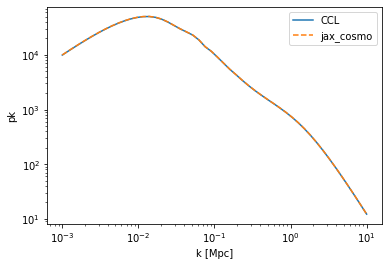
\includegraphics[width=\columnwidth]{figures/halofit_pk.png}
    \caption{Comparison of matter power spectrum between CCL and jax-cosmo. \textbf{Example of validation plot} \href{https://github.com/DifferentiableUniverseInitiative/jax_cosmo/blob/master/docs/notebooks/CCL_comparison.ipynb}{\faFileCodeO}}
    \label{fig:halofit_comparison}
\end{figure}



\section{Example of applications}
% illustrates why autodiff is interesting from several points of view

\subsection{DES Y1 setting}
% Here we describe the data and 3x2pt model for DES Y1 
 
In this section, we adopt as a setting a DES Y1 3x2pt-like analysis. 


\subsection{Instantaneous Fisher Forecasts}

\begin{minted}{python}
def likelihood(cosmo):
  # Compute mean and covariance of angular Cls, 
  # for specific probes
  mu, cov = gaussian_cl_covariance_and_mean(cosmo, 
                    ell, probes)
  # Return likelihood value
  return gaussian_log_likelihood(data, mu, cov)

# Compute derivatives of the likelihood with 
# respect to cosmological parameters
g = jax.grad(likelihood)(cosmo)

# Compute Fisher matrix of cosmological 
# parameters
F = - jax.hessian(likelihood)(cosmo)
\end{minted}

% Plot showing error in Jacobian computation by finite diff

% Plot showing error on some parameters

\subsection{Survey Optimization by FoM Maximization}
% Needs to mention the tomo challenge, mention that we can backpropagate through a NN and the cosmology model
% Maybe this can be only mentioned in the discussion.

\subsection{Massive Optimal Compression in 3 Lines}

% Here we can implement MOPED for the compression of 

\section{Gradient-based fast cosmological inference}
%
In the following sections we briefly review the statistical methods used to make some cosmological parameter inference. Namely we have used \textit{Stochastic Variational Inference} (aka SVI), \textit{Hybrid Hamiltonian Monte Carlo} (aka HMC), a variant of HMC knows as \textit{No-U-Turn} (aka NUTS), and finally the use of  \textit{Neural Transport}.   
%
\subsection{Stochastic Variational Inference}
%
Let us remind briefly what is the \textit{Stochastic Variational Inference} method \citep{2012arXiv1206.7051H, 2017arXiv171105597Z} and show where auto-differentiation helps. If one  writes $p(z)$ the prior, $p(\mathcal{D}|z)$ the likelihood and $p(\mathcal{D})$ the marginal likelihood, then thanks to the  Bayes theorem one gets $p(z|\mathcal{D})=p(z)p(\mathcal{D}|z)/p(\mathcal{D})$ the posterior distribution of a model with latent variables $z$ and a set of observations $\mathcal{D}$. The VI aims to get an approximation of this distribution, ie. $p(z|\mathcal{D}) \approx q(z;\lambda)$, by determining the variational parameters $\lambda$ of a predefined distribution. To do so, one uses the Kullback-Leibler divergence of the two distributions $KL(q(z;\lambda)||p(z|\mathcal{D}))$ leading to the following relation
\begin{align}
\log p(\mathcal{D}) &= \mathtt{ELBO} +  KL(q(z;\lambda)||p(z|\mathcal{D})) \label{eq-ELBO} \\
\mathrm{with} \ \mathtt{ELBO} &\equiv -\mathbb{E}_{q(z;\lambda)}\left[ \log q(z;\lambda)\right] + \mathbb{E}_{q(z;\lambda)}\left[ \log p(z,\mathcal{D}) \right] 
\end{align}
which defines the evidence lower bound (ELBO) that one tends to maximize to get the $\lambda$ values and the  highest lower bound on the logarithm of the marginal probability of the observations $\log p(\mathcal{D})$. So, the optimal variational distribution satisfies
\begin{equation}
q(z;\lambda^\ast) = \underset{q(z;\lambda)}{\mathrm{argmax}}\  \mathtt{ELBO} = 
\underset{\lambda}{\mathrm{argmin}}\ \mathcal{L}(\lambda)
\end{equation}
The function $\mathcal{L}(\lambda)$ is the cost function used in practice. It is composed of two parts:
\begin{equation}
\mathcal{L}(\lambda) = \underbrace{\mathbb{E}_{q(z;\lambda)}\left[ \log q(z;\lambda)\right]}_{guide} - \underbrace{\mathbb{E}_{q(z;\lambda)}\left[ \log p(z,\mathcal{D}) \right]}_{model}
\label{eq-loss-svi-1}
\end{equation}
where the \textit{guide} in the \numpyro\ library may be a multi-variate Gaussian distribution (MVN) for instance.

Using the auto-differentation tool, one can use "black-box" guides (aka \textit{automatic differentiation variational inference}). As stated by the authors of \citep{2016arXiv160300788K} ADVI helps specifying a variational family appropriate to the model, computing the corresponding objective
function, taking derivatives, and running a gradient-based or coordinate-ascent optimization. First is defined a bijective differentiable transformation $T$ of the original latent variables $z$ into new variables $\xi$, such $\xi=T(z)$ and $z=T^{-1}(\xi)$. One can develop "AutoGuides" (\numpyro\ terminology) that can be adapted to the user models. Then, the cost function reads
\begin{equation}
\mathcal{L}(\lambda) = \underbrace{\mathbb{E}_{q(\xi;\lambda)}\left[ \log q(\xi;\lambda)\right]}_{guide} - \underbrace{\mathbb{E}_{q(\xi;\lambda)}\left[ \log p(\xi,\mathcal{D}) \right]}_{model}
\label{eq-loss-svi-2}
\end{equation}
with
\begin{equation}
p(\xi,\mathcal{D}) \bydef p(T^{-1}(\xi),\mathcal{D}) |J_{T^{-1}}(\xi)|
\end{equation}
which exhibit the Jacobian of the $T^{-1}$ transformation. The main advantage of this reparametrisation is that the minimization can be performed with no bound constraints. 

Now, one is faced with the evaluation of the expectations during gradient descent. The solution is to use what is called \textit{elliptical standardisation} or \textit{re-parametrization trick} or \textit{coordinate transformation} (see references in \citep{2015arXiv150603431K}). Let us illustrate the trick in the case where $q(\xi; \lambda) = \mathcal{N}(\xi; \mu, \Sigma)$ ($\lambda=(\mu, \Sigma)$). One defines $S_\lambda$ such that $S_\lambda(\xi)=\zeta$, eg. $\zeta = L^{-1}(\xi-\mu)$ where $L$ is the Cholesky decomposition of $\Sigma=LL^T$. The Jacobien of this distribution is 1, so the cost function reads
\begin{multline}
-\mathcal{L}(\lambda) = \underbrace{\mathbb{E}_{\eta\sim \mathcal{N}(0,I)}\left[ \log p(T^{-1}(S_\lambda^{-1}(\zeta)),\mathcal{D}) + \log |J_{T^{-1}}(S_\lambda^{-1}(\zeta))| \right]}_{model} \\ + \underbrace{\mathbb{H}[q(\xi;\lambda)]}_{guide}
\label{eq-loss-svi-3}
\end{multline}
where $\mathbb{H}(q)$ is the Shannon entropy of the Gaussian distribution which is independent of the model, so its gradient can be computed once for all and reused in user model. Then,
to get $\nabla_\lambda \mathcal{L}$, the $\nabla$ operator can be put inside the expectation which leads to
\begin{multline}
-\nabla_\lambda\mathcal{L}(\lambda) = \mathbb{E}_{\zeta\sim \mathcal{N}(0,I)}\left\{
\left[ \nabla_z \log p(z,\mathcal{D}) \times \nabla_\xi[T^{-1}(\xi)] \right. \right. \\
+ \left. \left. \nabla_\xi \log|J_{T^{-1}}(\xi)| \right] \times \nabla_\lambda S_\lambda^{-1}(\zeta)
\right\}
+ \nabla_\lambda \mathbb{H}[q(\xi;\lambda)]
\label{eq-loss-svi-4}
\end{multline}
For the use case of the MVN (auto)guide, one gets
\begin{align}
-\nabla_\mu \mathcal{L} &= \mathbb{E}_{\zeta\sim \mathcal{N}(0,I)}\left\{
\nabla_z \log p(z,\mathcal{D}) \times \nabla_\xi[T^{-1}(\xi)]
+ \nabla_\xi \log|J_{T^{-1}}(\xi)|
\right\} \nn \\
-\nabla_L \mathcal{L} &= \mathbb{E}_{\zeta\sim \mathcal{N}(0,I)}\left\{
\left[ \nabla_z \log p(z,\mathcal{D}) \times \nabla_\xi[T^{-1}(\xi)] \right.\right. \nn\\
&\left. \left. \qquad\qquad\qquad + \nabla_\xi \log|J_{T^{-1}}(\xi)| \right] \times \xi^T 
\right\}+ (L^{-1})^T
\end{align}
The expectations used in the above expressions are computed with $\zeta$ i.i.d samples from $\mathcal{N}(0,1)$ distribution which reveals the "S" of SVI. Even, if one can sample from the optimized  $q(z,\lambda^\ast)$ distribution, we have used SVI as front-end to  a NUTS sampler which is described in section \ref{sec-Neural-Reparametrisation} as \textit{Neural Transport}.
%
\subsection{Hamiltonian Monte Carlo}

\subsubsection{Introduction}

% Show Joe's vanilla HMC results against Cobaya
Hamiltonian Monte Carlo (HMC) is an MCMC-type method particularly suited to drawing
samples from high dimensional parameter spaces.  It was introduced in \citep{1987PhLB..195..216D}
and developed extensively since.  See \citet{betancourt} for a full review; we describe
very basic features here.

HMC samples spaces by generating particle tracjectories through the space, using the log-posterior
as the negative potential energy of a particle at each point $q$ in the space.  At each sample a trajectory are initialized
with a random momentum $p$, and then integrated using Hamilton's equations with a numerical integration:
\begin{align}
\frac{\mathrm{d}p}{\mathrm{d}t} &= - \frac{\partial V}{\mathrm{d} q} = \frac{\partial \log{\cal P}}{\mathrm{d} q}\\
\frac{\mathrm{d}q}{\mathrm{d}t} &= + \frac{\partial U}{\mathrm{d} p} = M^{-1} p
\end{align}
where $M$ is a mass matrix which should be set to approximate the covariance of the posterior. This is also
used to set the scale of the random initial velocities.

Formally, the set of $n_\mathrm{dim}$ moment are treated as new parameters, and after 
some number of integration steps a final point in the trajectory is compared to the initial one,
and a Metropolis-Hastings acceptance criterion on the total energy $H = p^T M^{-1} p + \log{\cal P}(q)$ is applied.
If the trajectory is perfectly simulation then this acceptance is unity, since energy is conserved; applying it allows
a relaxation to the integration accuracy.

That gradients $\partial \log{\cal P} / \mathrm{d} q$ can be estimated using finite differencing,
but this typically requires at least $4 n_{\mathrm{dim}} + 1$ posterior evaluations per point, greatly slowing it
in high dimension, and as with the Fisher forecasting is highly prone to numerical error. Automatically
calculating a Hessian, as in JAX-Cosmo, makes it feasible and efficient.

Below we show an example set of HMC constraints using JAX-Cosmo to constrain a simulated
Dark Energy Survey Year One (DES-Y1) lensing and clustering-like (3x2pt) likelihood, using 21 parameters\footnote{We omit the 
five clustering sample photometric redshift parameters}.  We re-parametrize the space to unit mass using the Cholesky 
decomposition
of the covariance as estimated with an initial Fisher matrix; this lets us reflect the trajectories when they reach the
edge of the parameter space, as recommended in \citep{NIPS2015_8303a79b}.  We use a fixed number (25) of integration steps and 
a fixed integration period (0.02), this was chosen heuristically to give a reasonable acceptance rate, but is likely to be
far from optimal.  We compare to the highly-optimized {\sc Cobaya} 
Metropolis-Hastings implementation \citep{cobaya2,cobaya1}, initializing it with the Fisher matrix as a proposal and
tuning thereafter.  We ran two processes for each sampler, with four CPU threads per process.

The Hamiltonian sampler required around half the number of samples as the Metropolis (70,000 vs 140,000) to reach approximately the same
convergence, as tested by the Gelman-Rubin test \citep{gelman}, though each sample was itself a few times slower
on a CPU.  This proof-of-principle example can certainly be hugely improved using various extensions to HMC such as No U-Turn Sampling \citep{nuts} or sampling from the entire trajectories \cite{betancourt}.  On next generation GPU high-performance systems, the advantage will be large.

\begin{figure}
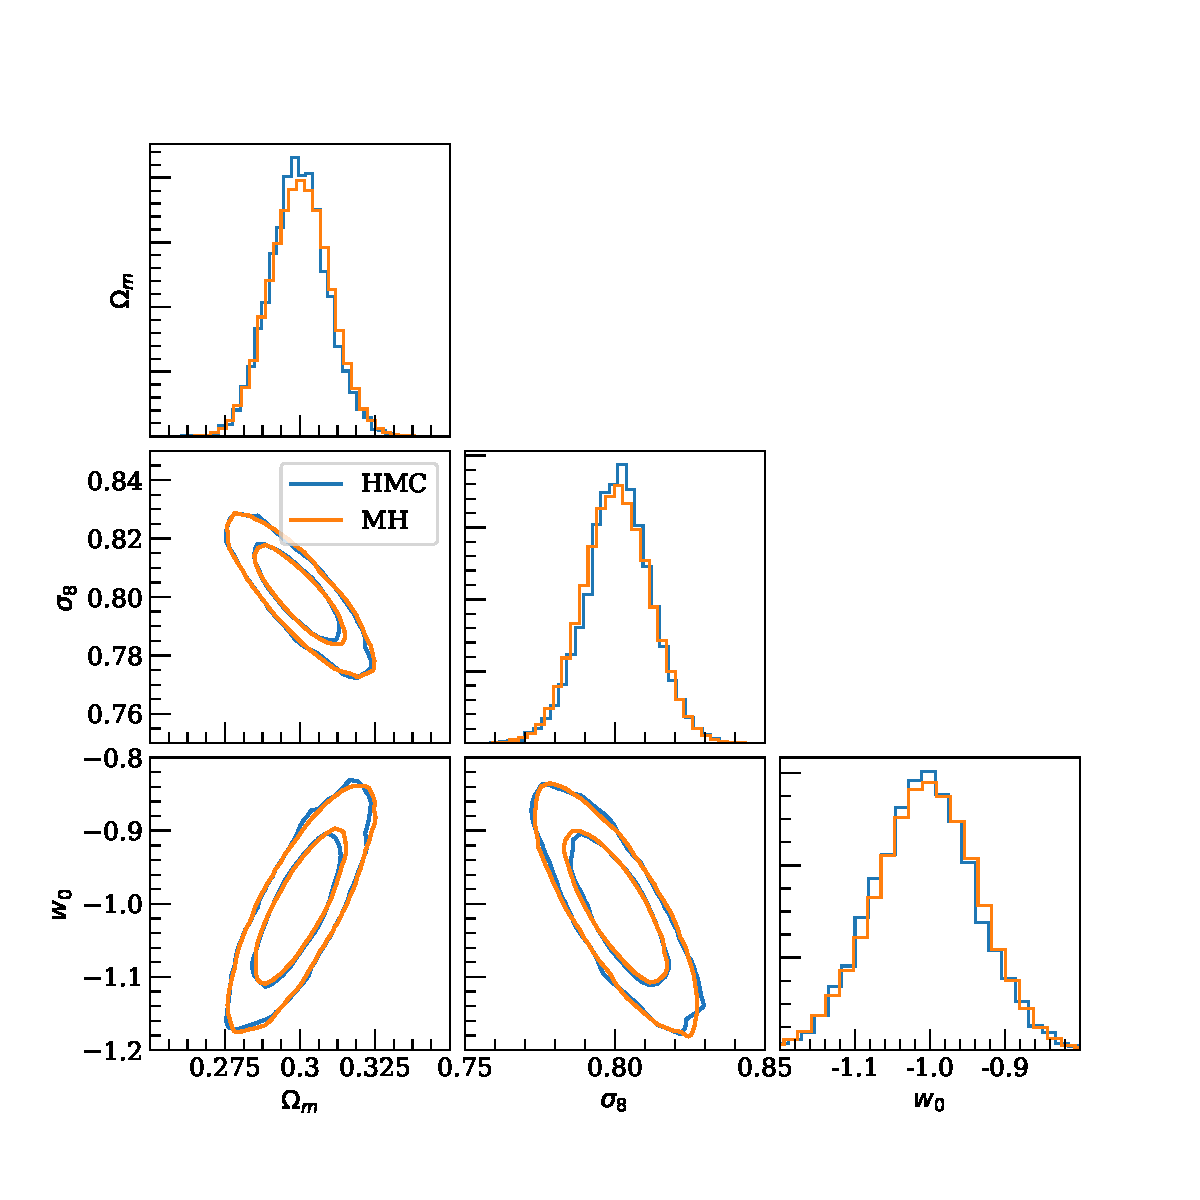
\includegraphics[width=0.95\columnwidth]{figures/hmc.pdf}
\caption{Constraints on three of the 21 parameters of a simulated DES-Y1 3x2pt likelihood, using a simple Hamiltonian
Monte Carlo sampler with JAX-Cosmo (blue), compared to the Cobaya Metropolis-Hastings sampler (orange).}
\end{figure}


We note that a full Boltzmann code accurate enough to calculate the CMB spectra to Planck \citep{planck18}
or future \citep{s4,simons} accuracy is currently beyond the scope of this project.  
If this is needed then HMC could use a fast approximation to a CMB theory spectrum, and importance sampling applied to the complete chain.

\subsubsection{NUTS}
\label{sec-NUTS}
%
% Show the advantage of using NUTS 
% look at difference in efficiency in terms of how many times we need to call the model.

A variant of the traditional HMC sampler has been introduced in reference \citep{nuts}. It aims to help finding a new point  $x_{i+1}$ from  the current $x_i$. Namely, the root algorithm of HMC deals with the \textit{leapfrog} integration which requires to set two main parameters: $\varepsilon$ the step size and $L$ the number of steps. As stated by the authors, NUTS  uses a recursive algorithm to build a set of likely candidate samples that spans a wide swath of the target distribution, stopping automatically when it starts to double back and retrace its steps. So, in a automatic manner the parameter $L$ is adjusted to produce statistically  a new point $x_{i+1}$ independent from $x_i$, at the expense of the increase the number of model calls. The user has to set a new  parameter  (\texttt{max\_tree\_depth}) which gives in power of $2$ the maximal number of model calls a each generation.

Both sampler HMC and NUTS are available in the \numpyro\ library: \texttt{NUTS} is inherited from \texttt{HMC} which in turns is inherited from the generic \texttt{MCMC} class. So, We have setup \texttt{NUTS} sampler Using the same DES-Y1 modeling as in previous section, with 
\begin{itemize}
    \item first a reparametrisation of the latent variable uniform priors (Tab.~\ref{tab-DESY1}) to use a unified uniform prior $\mathcal{U}[-5,5]$;
    \item second for the warm-up phase we ask for mass matrix optimisation with essentially a diagonal form but with a block structure for the following sets of parameters $(\Omega_b,\Omega_c,\sigma_8,w_0,h)$ and $(b_i)_{i:1\dots5}$. This matrix structuring is motivated by the expected degree of correlation of the concerned parameters as can be shown for instance in figure \ref{fig_svi_nuts_4}.
\end{itemize}
We have setup a NUTS sampling using 16 chains of 1,000 samples each (\texttt{vectorized} option) after a warm-up phase consisting of 200 samples and the \texttt{max\_tree\_depth} has been set to 7 by default (ie. 128 steps for each iteration). The job has been undertaken on a single GPU either a NVidia Titan Xp (12GB RAM) on a desktop or NVidia V100 (32GB RAM) at the CCIN2P3 Center.

The results in terms of sampling efficiency are detailed in Tab.~\ref{tab-ESS-NUTS_SVI-1}. The confidential level iso-contours are all in agreement with the \texttt{cobaya} sampler and are reported as the blue curves in figures presented in section \ref{sec-Neural-Reparametrisation}. It is worth to point out that the mass matrix structuring is a very effective when NUTS is run stand-alone as it increases the sampling efficiency by about a factor 2.  The elapse time was 20 hours for the default setting (\texttt{max\_tree\_depth=7}). Anticipating the section \ref{sec-Neural-Reparametrisation} devoted to the Neural Transport which is an effective alternative, we have used a NUTS sampling with \texttt{max\_tree\_depth=5} those elapse time is 5 hours. This clearly shows a linear scaling with respect to the number of steps per iteration keeping the sampling efficiencies at a high level (see Tab.~\ref{tab-ESS-NUTS_SVI-1}), so the user is highly encouraged to tune this critical parameter. 
 
%  JEC: the 16 chains X 1000 (max_tree_depth=7) is the run done by Francois. 20 heures sur un GPU TitanXp avec 12 GB de ram 
% 5h sur V100 10 chains x 1000 (max_tree_depth=5)

%
\subsubsection{Neural Transport}
\label{sec-Neural-Reparametrisation}
%
If the SVI method can be used as is to get $z$ i.i.d. samples from the $q(z,\lambda^\ast)$ distribution, the \textit{Neural Transport MCMC} method \citep{2014arXiv1412.5492P,2019arXiv190303704H} is an efficient way to boost HMC efficiency, especially in target distribution unfavourable geometry where for instance the leapfrog integration algorithm has to face squeezed join distributions for a subset of variables. From SVI, one obtains a first approximation of the target distribution and we show that the change-of-variable $z=F_\lambda(\zeta)$ is such that
\begin{equation}
q(z;\lambda) \rightarrow q(\zeta;\lambda) \bydef q(F_\lambda(\zeta)) |J_{F_\lambda}(\zeta)|
\end{equation}
which is evaluated with optimal $\lambda^\ast$ according to maximization of the ELBO (eg. $F_\lambda=T^{-1}\circ S^{-1}_\lambda$). So, one can use a HMC sampler (eg. NUTS) based on $p(\zeta;\mathcal{D})$ distribution, initialized with $\zeta$ samples from $q(\zeta;\lambda^\ast)$, to get a Markov Chain of $N$ samples $(\zeta_i)_{i<N}$. Then, from the transformation  $z_i=F_{\lambda^\ast}(\zeta_i)$ one finally obtain a Marcov Chain with $(z_i)_{i<N}$ samples. The method is accessible throw the \verb|NeuTraReparam| in \numpyro\ library.

\begin{figure}
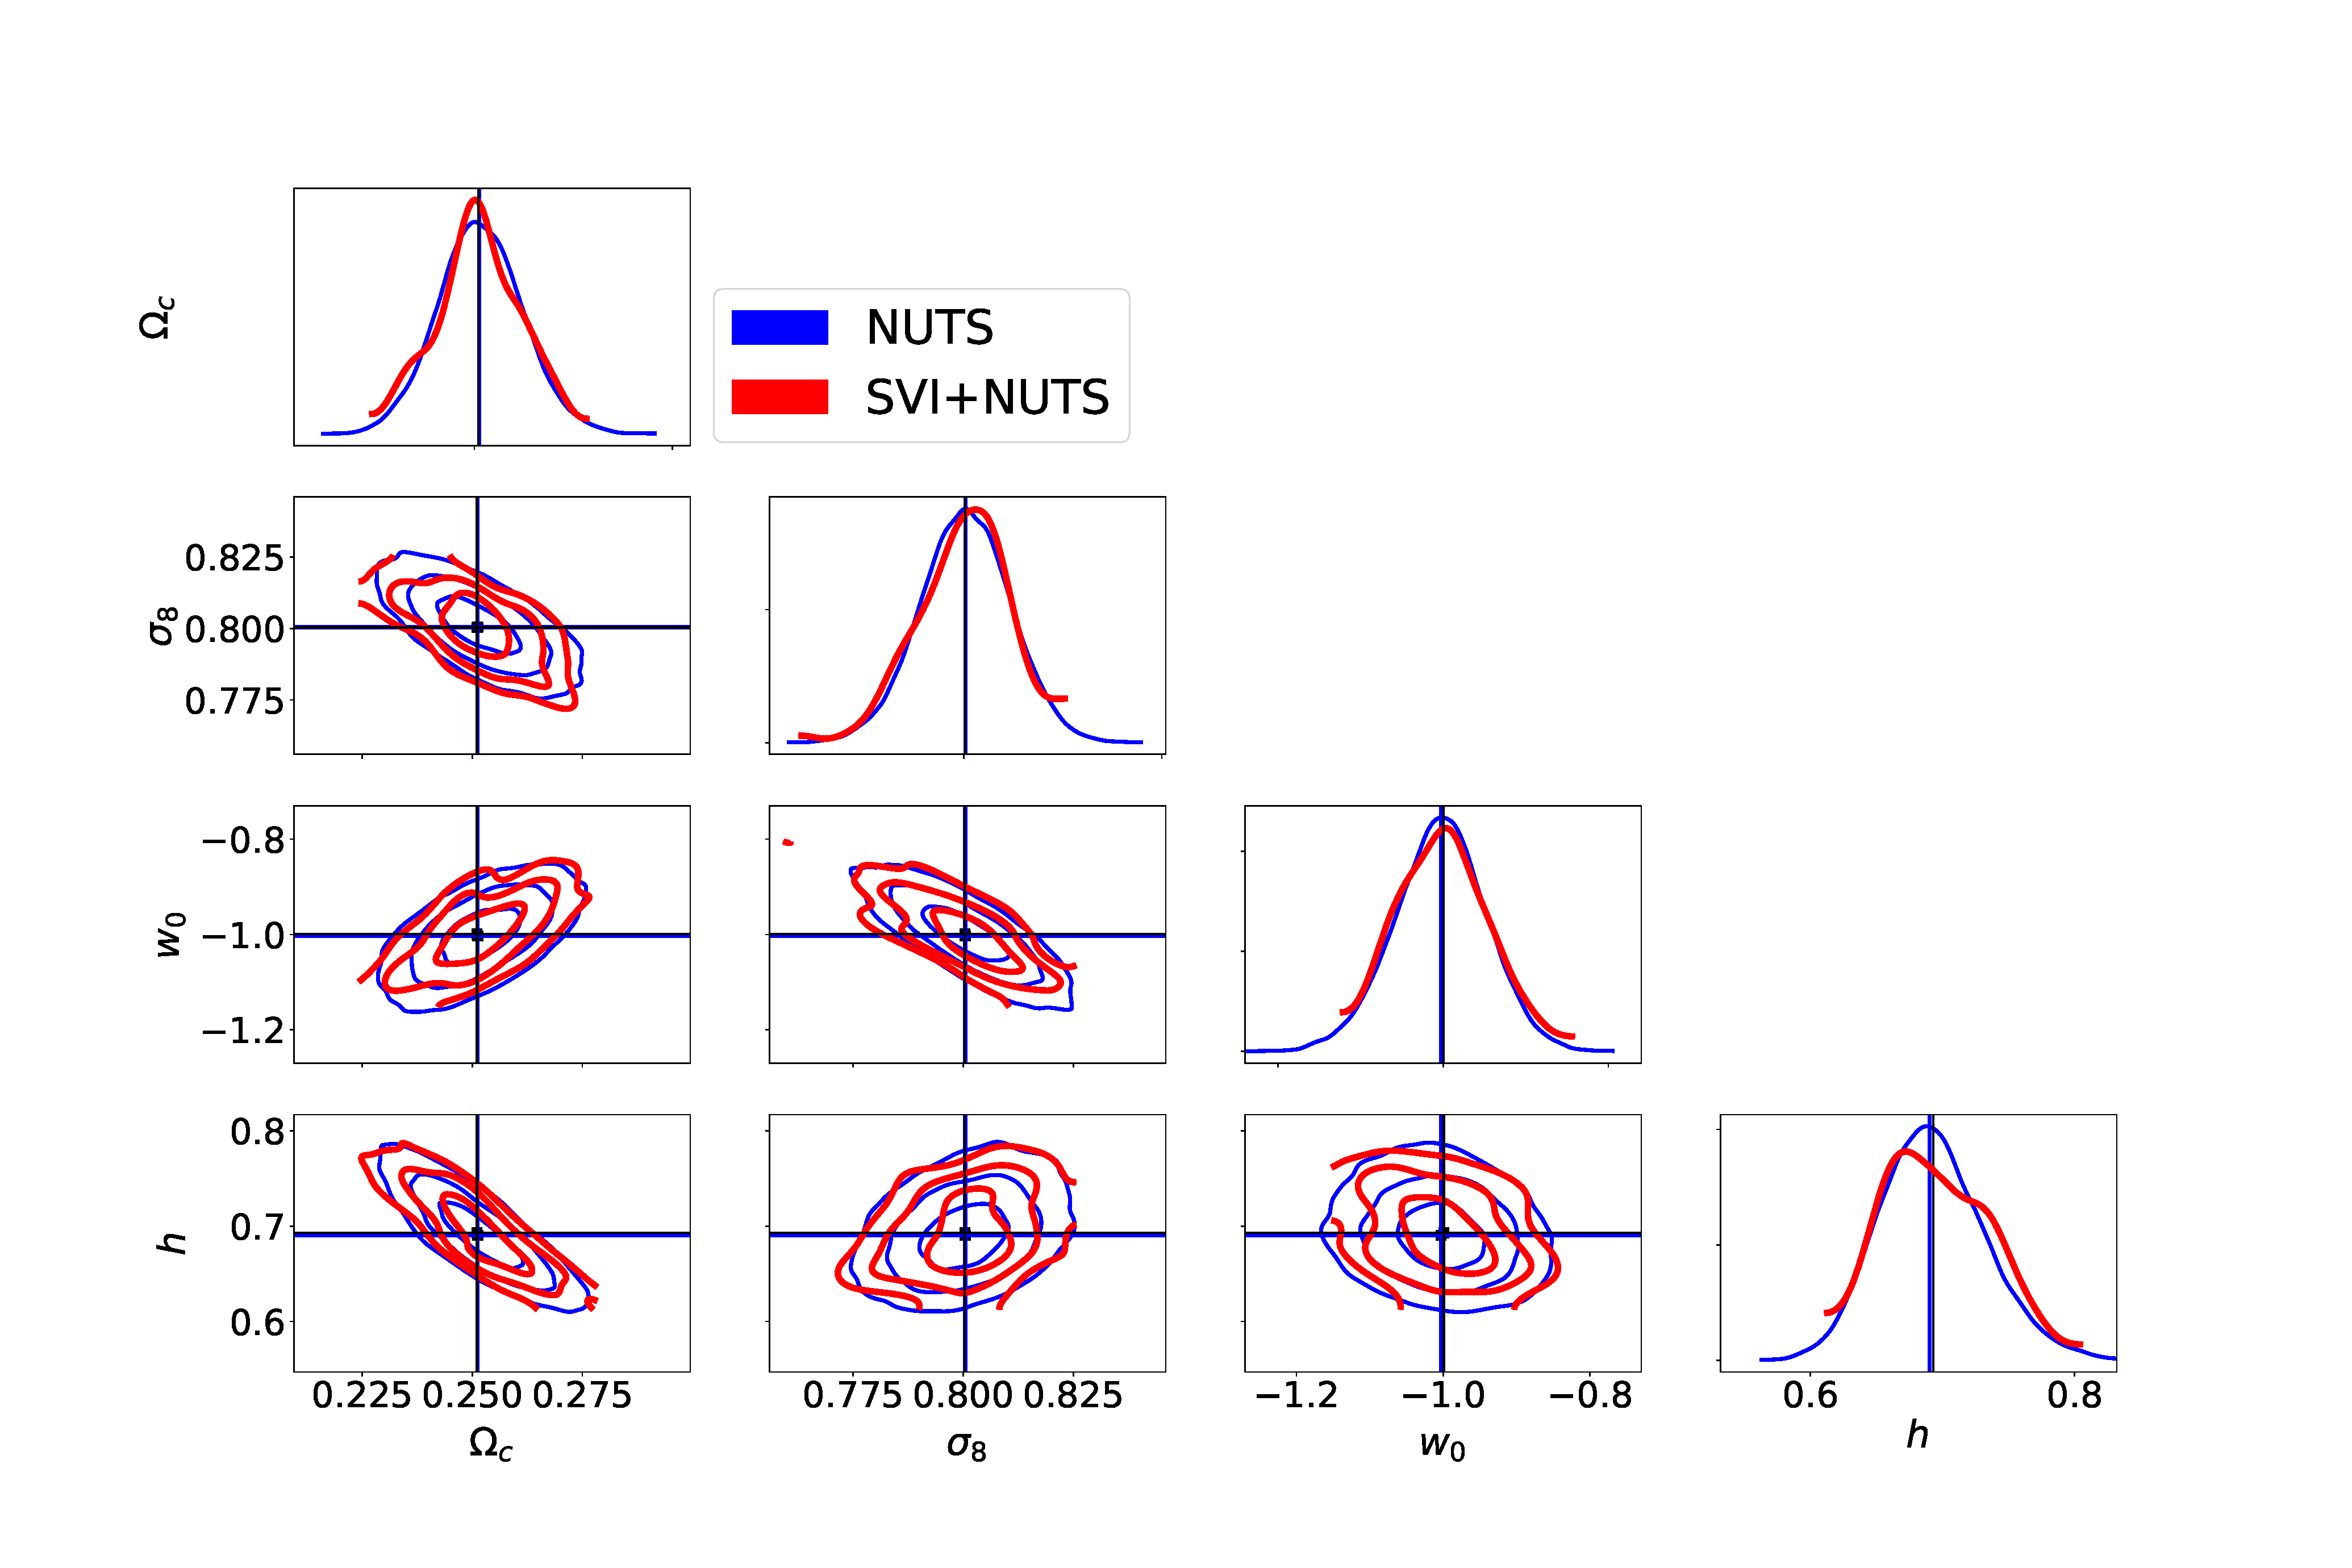
\includegraphics[width=\columnwidth]{figures/SVI_NUTS_1x200x200.pdf}
\caption{Constraints (30\%, 68\%, 90\%) on 4 of the 22 parameters of a simulated DES-Y1 3x2pt likelihood, in blue the NUTS sampling described in section \ref{sec-NUTS}, and in orange a SVI MVN optimisation followed by a Naural Transport parametrisation to run a NUTS sampling (1 chain of 200 warm followed by 200 samples; a dense mass matrix and \texttt{max\_tree\_depth} parameter set to 5).}
\label{fig_svi_nuts_1}
\end{figure}

\begin{figure}
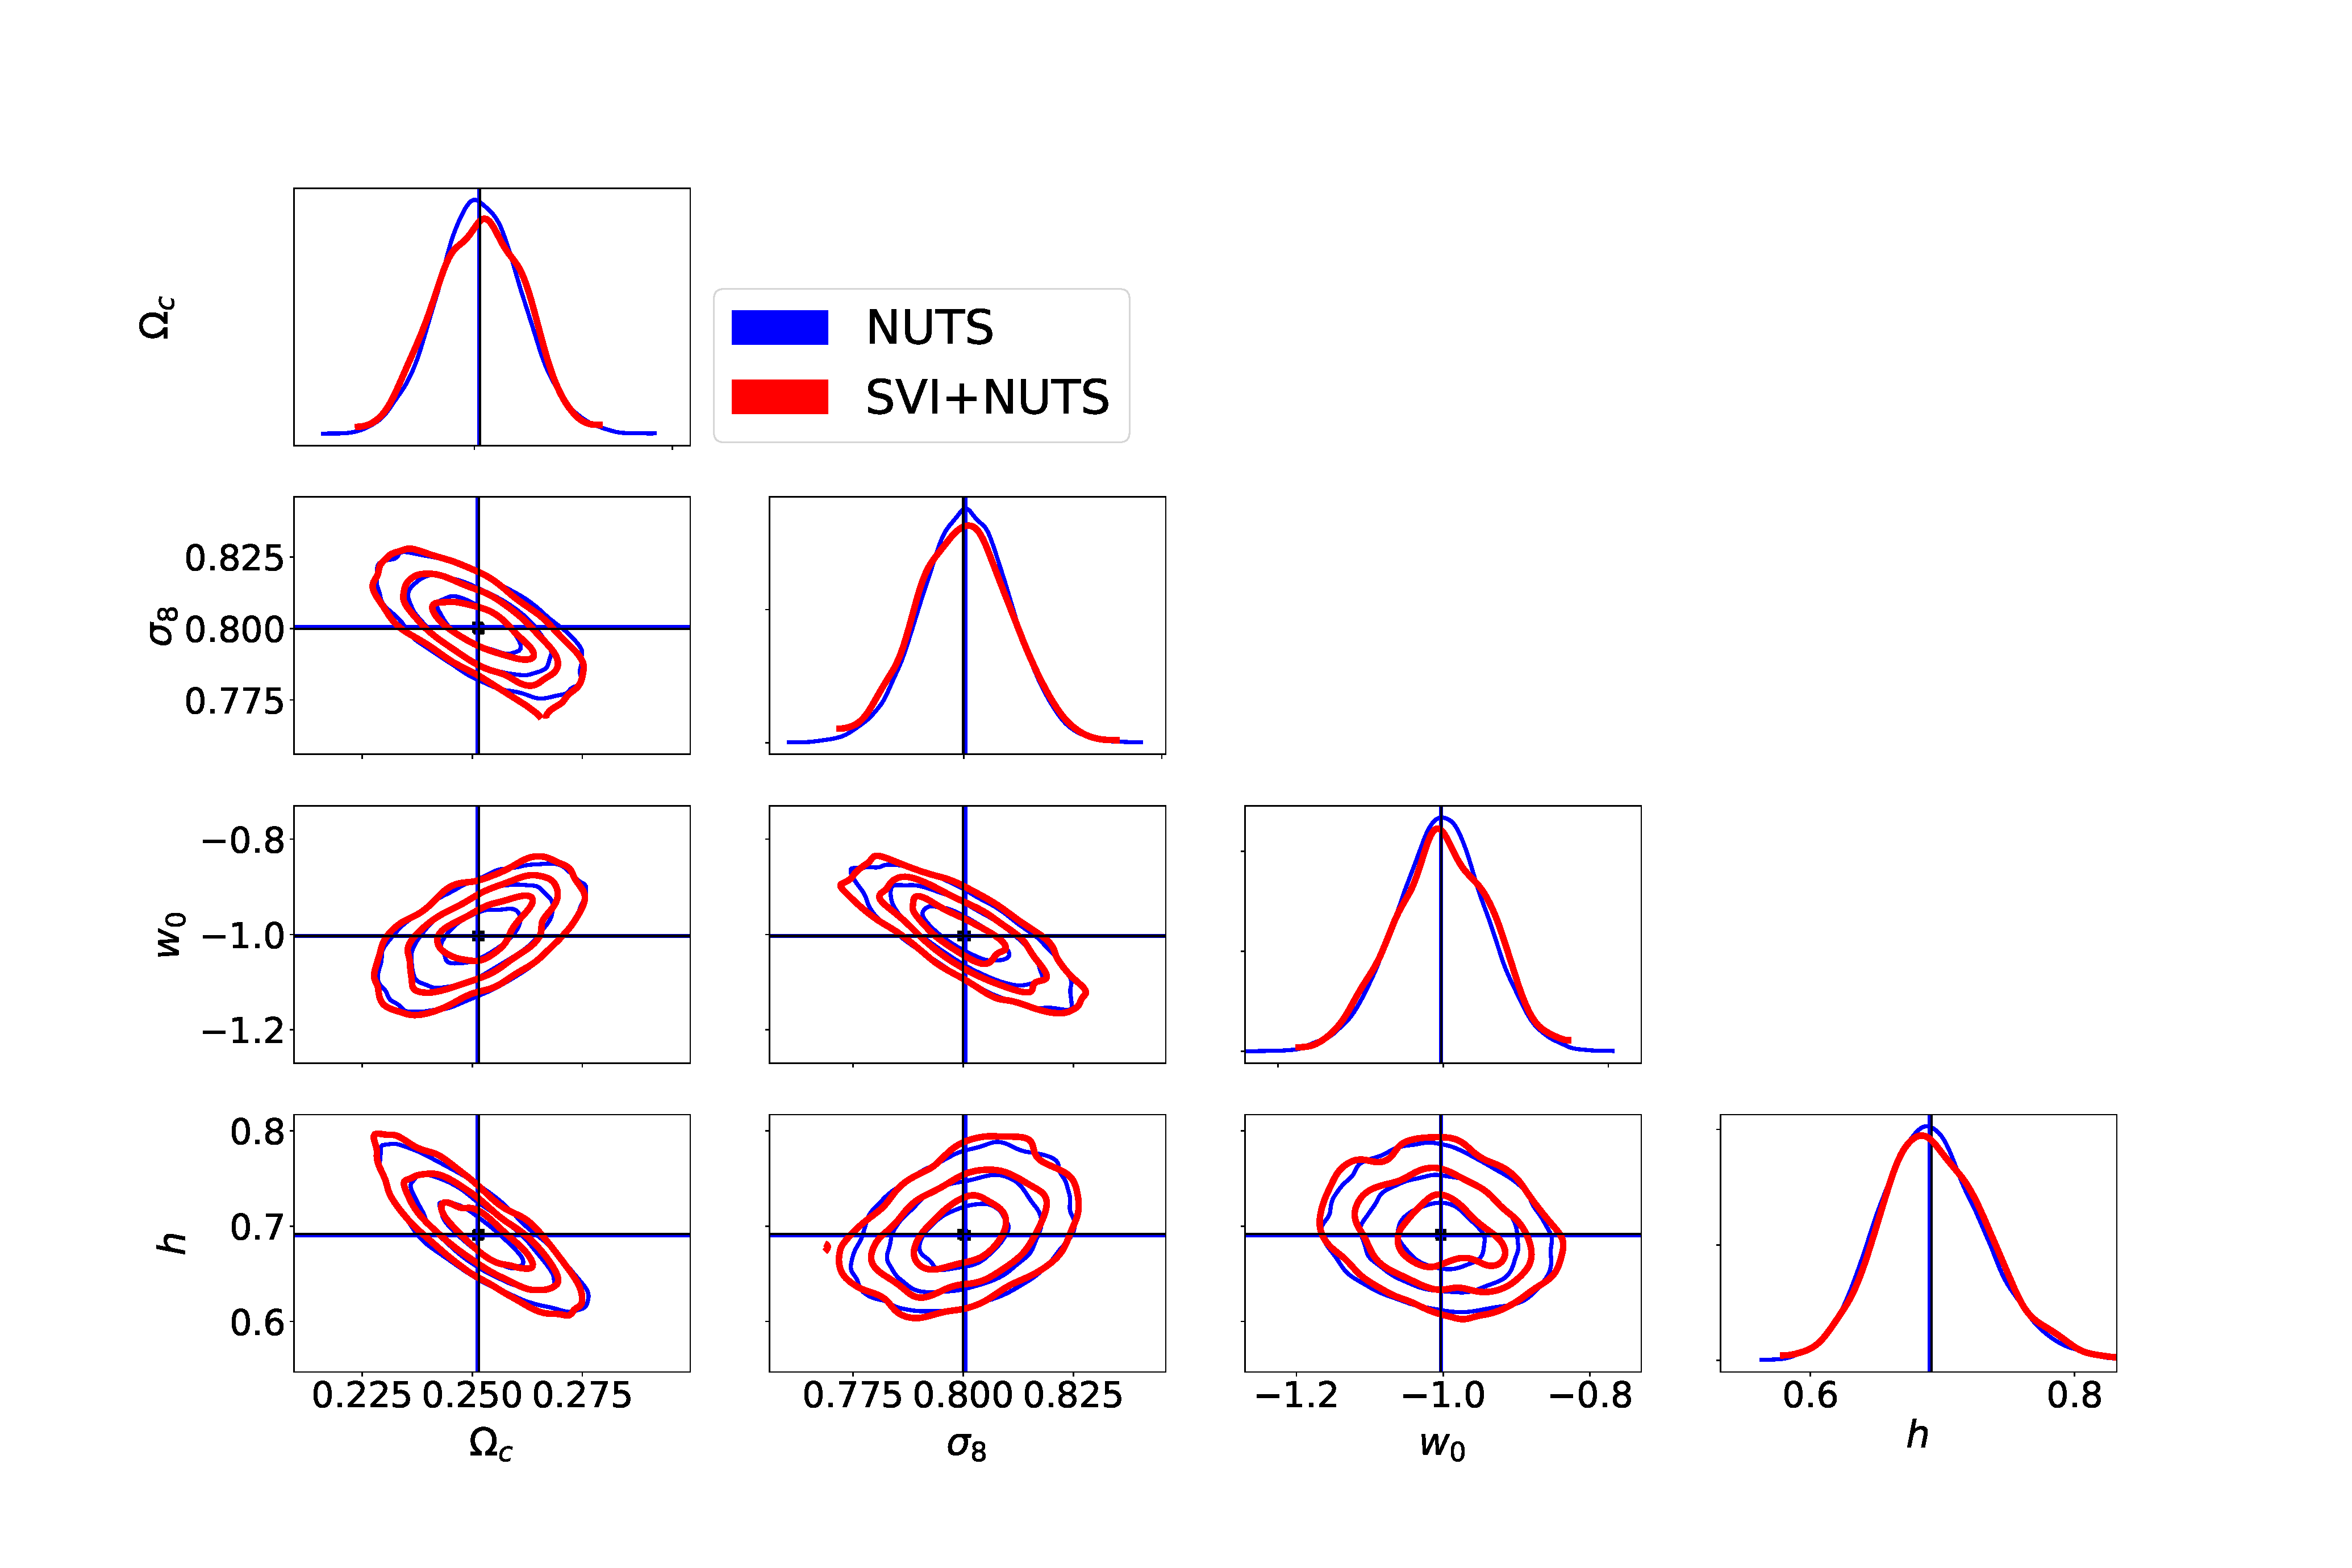
\includegraphics[width=\columnwidth]{figures/SVI_NUTS_1x200x1000.pdf}
\caption{Same as Fig.~\ref{fig_svi_nuts_1} but with 1 chain of 200 warm followed by 1000 samples for the NUTS sampler after SVI optimization.}
\label{fig_svi_nuts_2}
\end{figure}

\begin{figure}
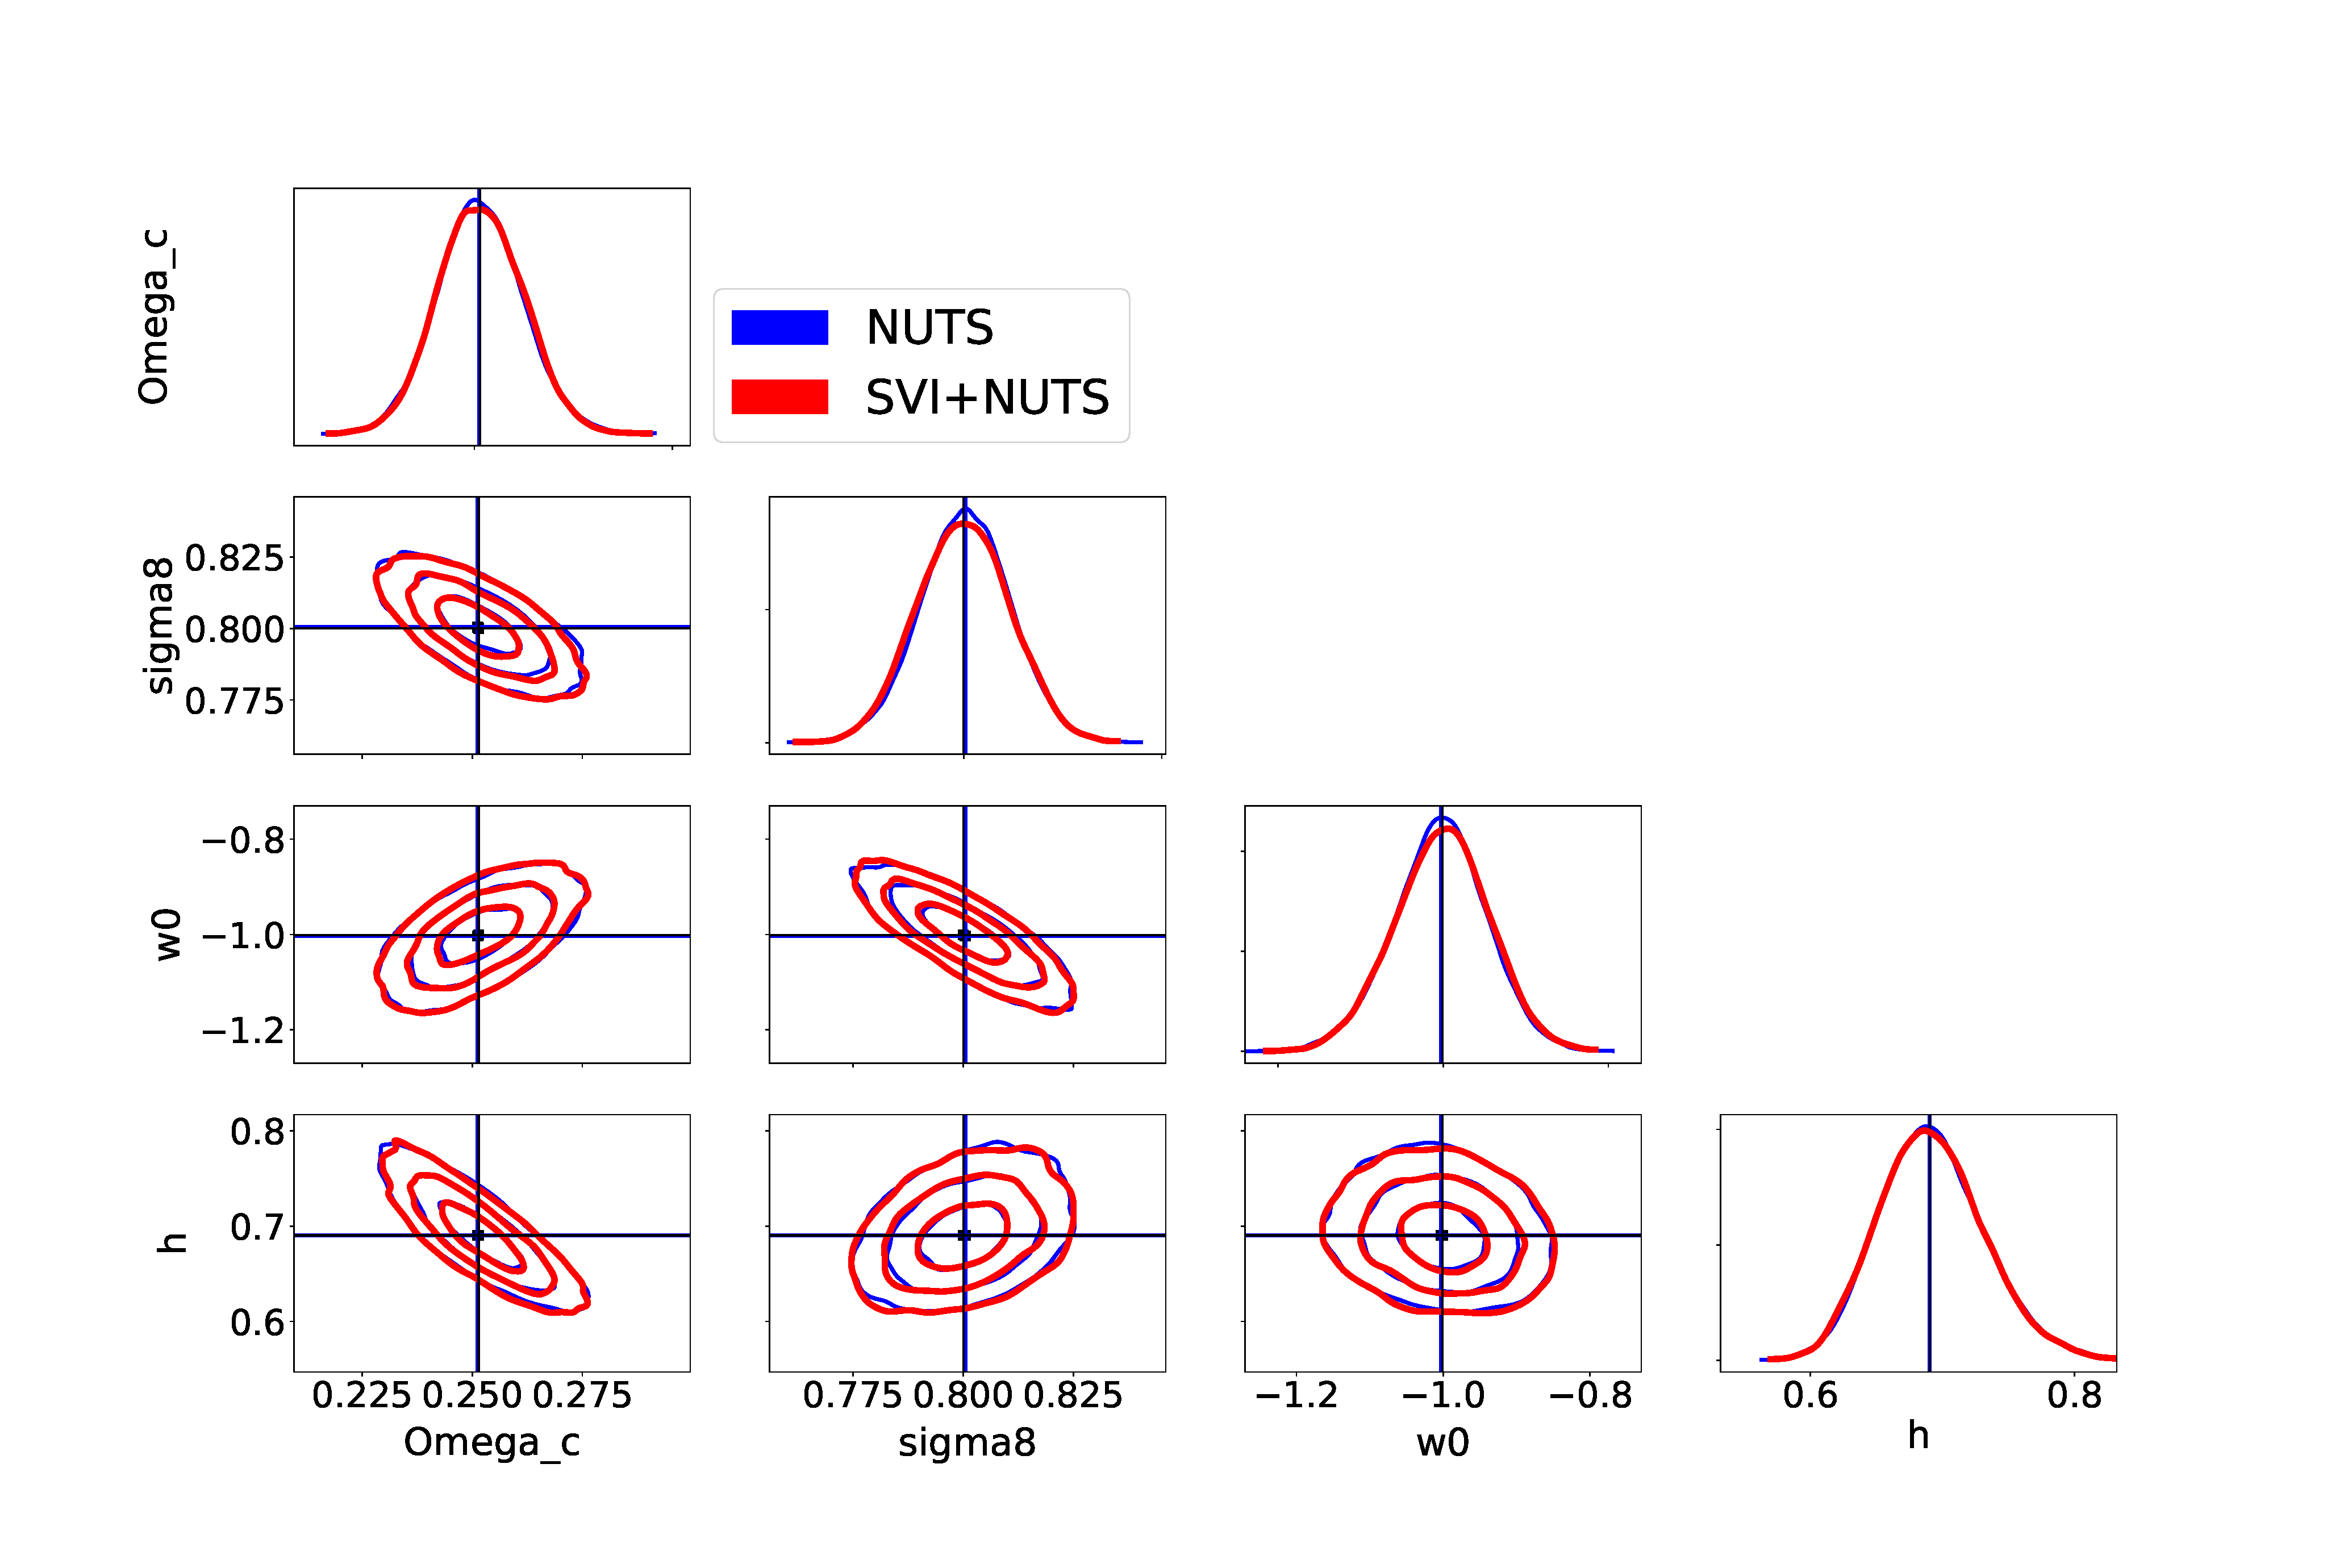
\includegraphics[width=\columnwidth]{figures/SVI_NUTS_10x200x1000.pdf}
\caption{Same as Fig.~\ref{fig_svi_nuts_1} but with 10 chains of 200 warm followed by 1000 samples for the NUTS sampler (\texttt{max\_tree\_depth=5}) after SVI optimization.}
\label{fig_svi_nuts_3}
\end{figure}

\begin{figure}
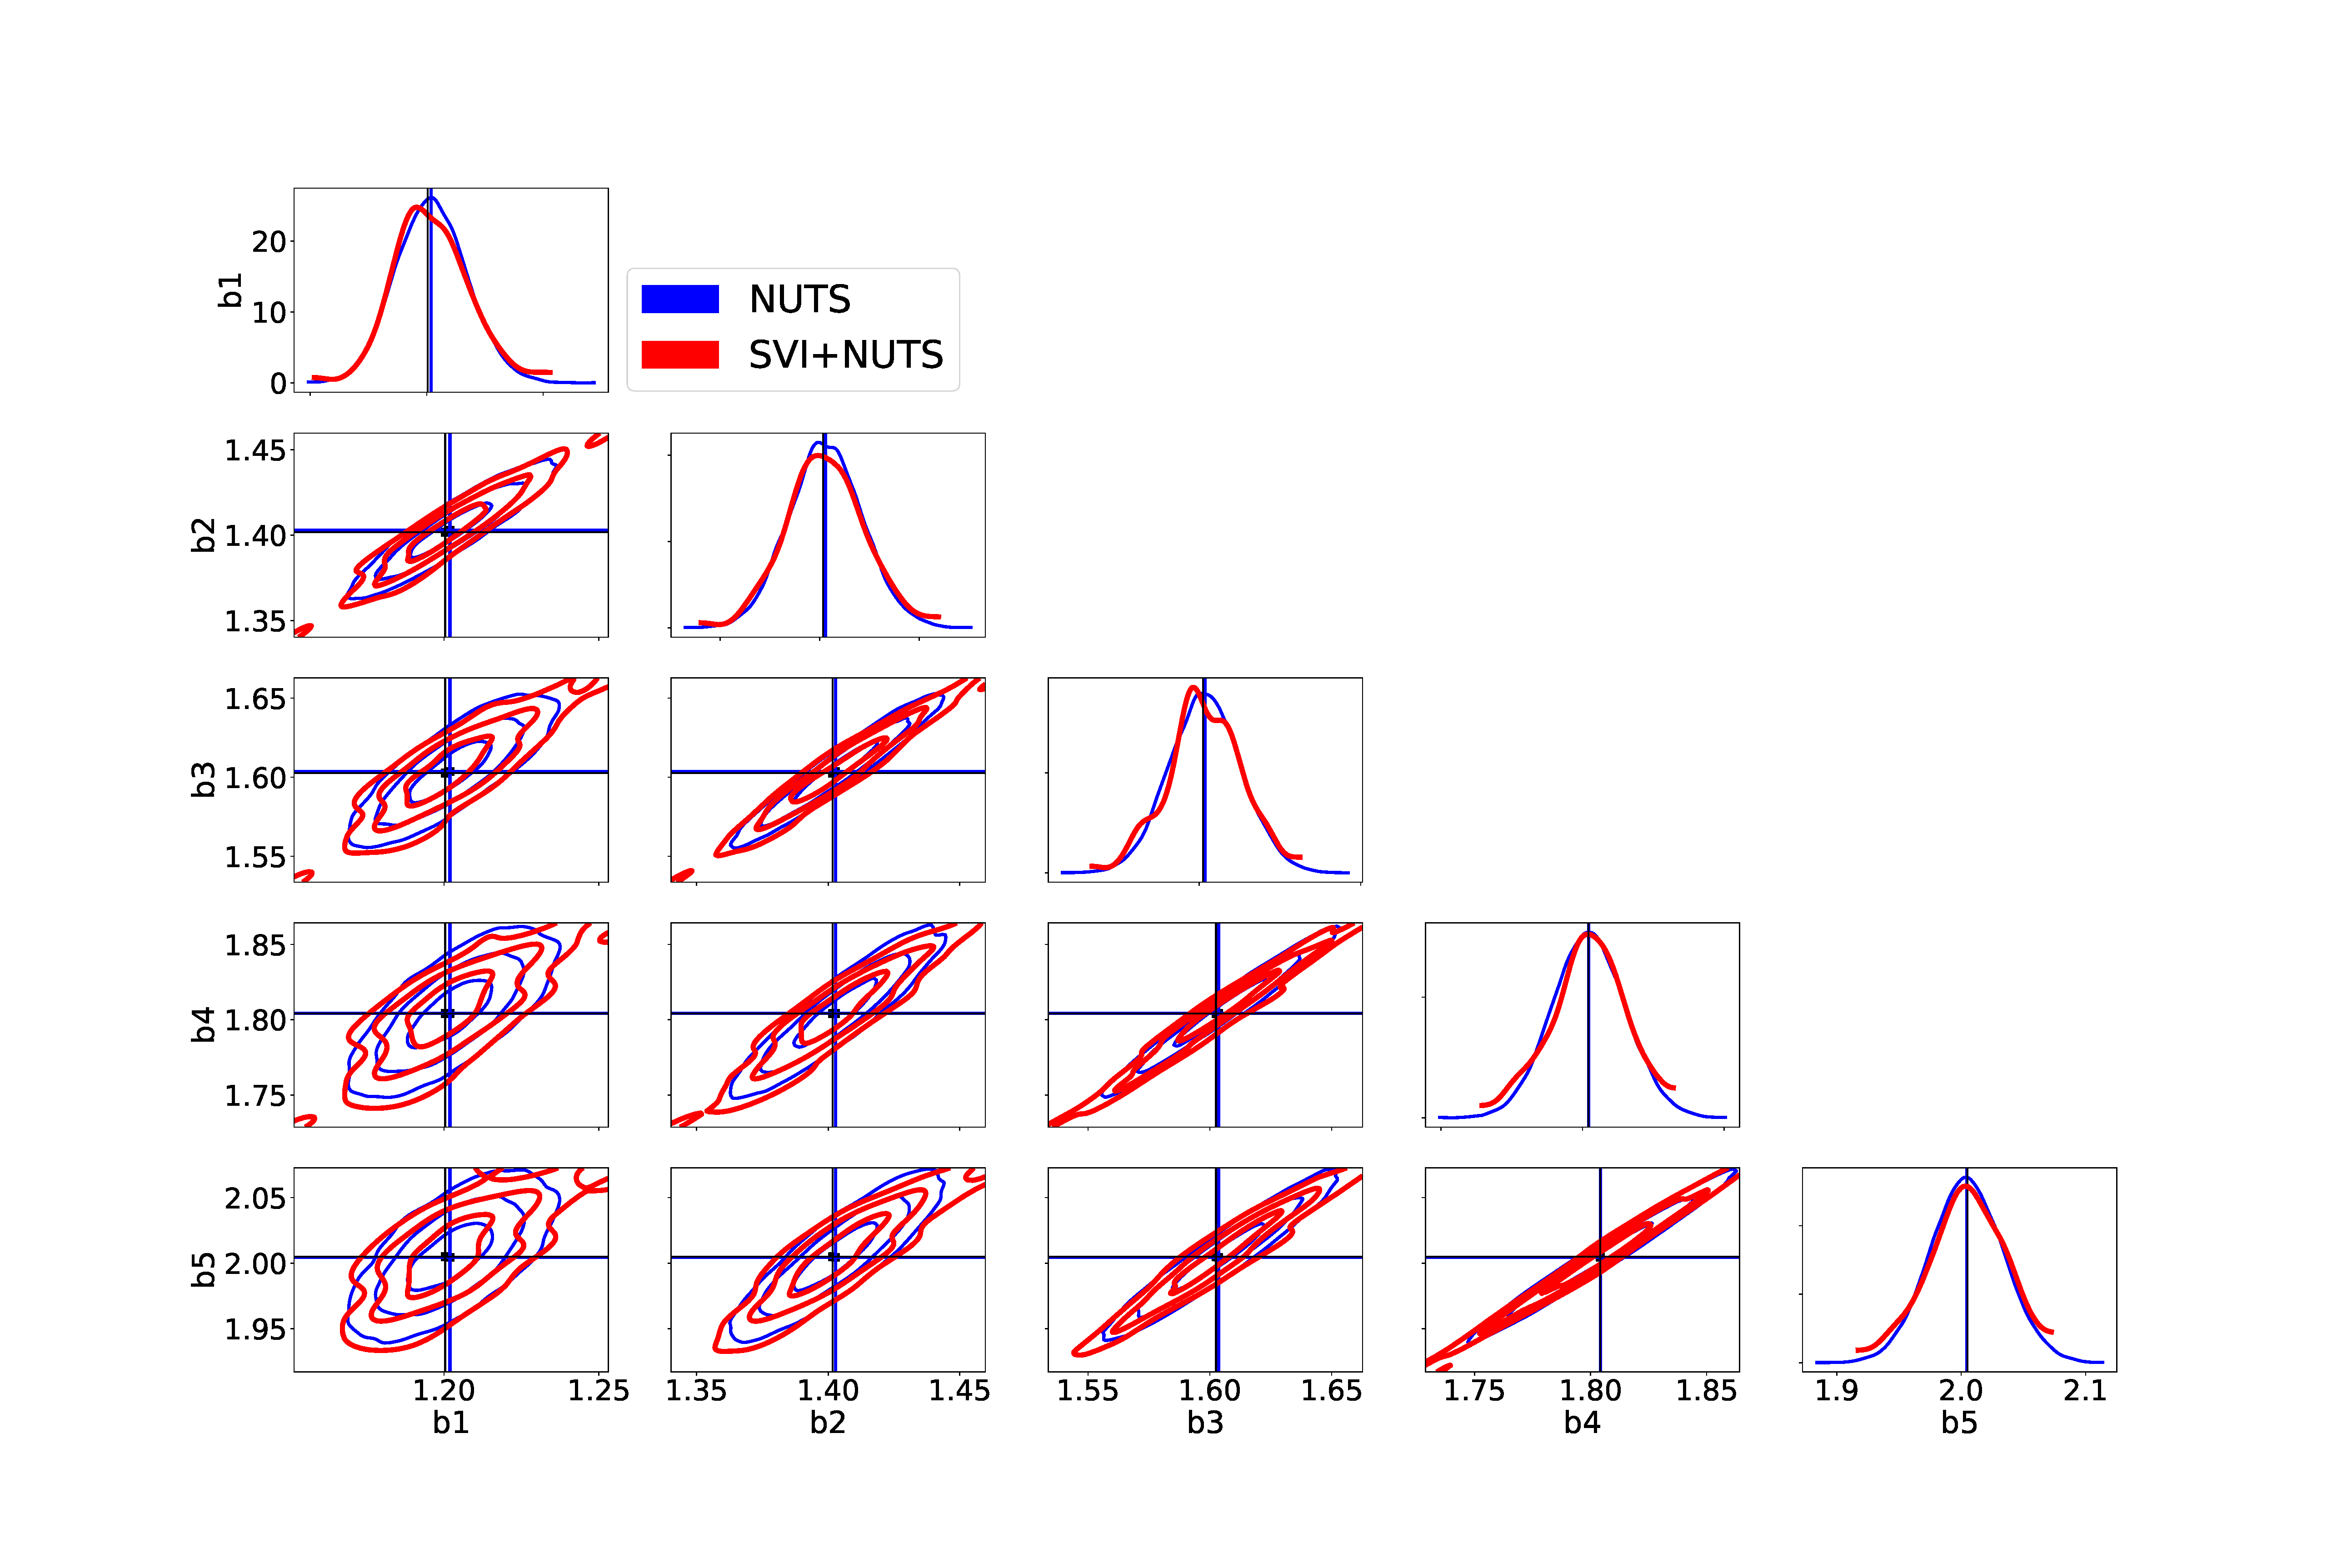
\includegraphics[width=\columnwidth]{figures/SVI_NUTS_1x200x200_bis.pdf}
\caption{In the same conditions of Fig.~\ref{fig_svi_nuts_1} but for the five lens galaxy bias which are highly correlated.}
\label{fig_svi_nuts_4}
\end{figure}


Using the same DES-Y1 simulation as in previous section, we have used the \numpyro\ library to first use a simple Multivariate Normal distribution as \textit{guide} to approximate the true posterior (\textit{model}) to feed a SVI. The Adam optimizer has been used with a learning rate set to $10^{-3}$.  Then, we have used the Neural Transport method to generate Markov Chains of different sizes by the NUTS sampler. The SVI optimization requires 20,000 steps and has been performed in about 2 hours on a Nvidia V100 GPU (32 GB RAM). Concerning the NUTS running on the same GPU, the chains have run 200 warm samples, and then 200 samples, 1000 samples on a single chain, and finally we have run 10 chains (\texttt{vectorized} option) with 1000 samples each. All NUTS sampling as been performed with dense mass matrix optimisation without special block structuring and with \texttt{max\_tree\_depth=5} which is different than the default NUTS setting described in section \ref{sec-NUTS}. 

The elapse time for each of these 3 runs is 50 minutes, 150 minutes and 5 hours, respectively. The results of the evolution of the 2D parameters contour levels compared to the default NUTS sampling (Sec.~\ref{sec-NUTS}) are displayed in figures \ref{fig_svi_nuts_1}, \ref{fig_svi_nuts_2}, \ref{fig_svi_nuts_3}. The agreement is rather good even for the highly correlated $(b_i)_{i:1,\dots,5}$ bias parameters as show on figure \ref{fig_svi_nuts_4}. Results in terms of sampling efficiency are shown on Tab.~\ref{tab-ESS-NUTS_SVI-1} showing that the SVI followed by Neutral Parametrisation gives high efficiency as well without the need by the user to setup a particular mass matrix structuring (ie.\texttt{dense} matrix option). 
%
\subsection{Discussion}
%
The question that one may naturally arises are what is the HMC/NUTS gain compared to the well known standard \texttt{cobaya} sampler? 
In one hand, one may argue considering the elapse time of execution that the number of efficient sample per model call is a right metric to consider: 
\begin{equation}
    \eta = \frac{n_{eff}}{\#\ of\ calls} = \frac{N_s \times \varepsilon}{N_s \times n_{steps}} = \frac{\varepsilon}{n_{steps}}
\end{equation}
with $N_s$ the total number of samples, $\varepsilon$ the sampler efficiency and $n_{steps}$ the number of steps (calls) per sample generation. Then, for \texttt{cobaya} one roughly gets $\varepsilon\approx 1\%$ with $n_{steps}=1$ while for the NUTS sampler $\varepsilon\approx 50\%$ but at the expense of $n_{steps}=2^5$ or more. At the end of the day, the $\eta$ values for both methods are comparable (ie. about $1\%$). So, at first sight considering the elapse time that there might be no gain to use HMC/NUTS sampler compared to standard MCMC sampler.  

On the other hand, the above metric is one aspect of the sample generation. One should have in mind that the low sampling efficiency of standard MCMC sampler requires mobilizing a large amount of resources to produce a sufficient large sample batch in a reasonable time scale, ie. several days on dedicated infrastructure. Moreover, the user is faced to a dilemma to perform or not a statistical sample selection post-processing as \textit{thinning} beyond the \textit{burn-in removal} which is a rather delicate procedure and time consuming too, needing how-know to be conducted correctly \citep{doi:10.1146/annurev-statistics-040220-091727, 2015arXiv151007727O}. So, the authors think that it is worth considering methods that by construction are more efficient. Moreover, using SVI with neural reparametrisation offers an effective way to undertake a progressive validation of the model with rather modest sample size (eg. 200 samples) by producing good quality marginal contours in few hours. In practice, this validation phase can save time before producing sizeable batch for final analysis. The authors have not investigated very high dimensional ($O(10^2)$ parameters) as well as multi-modal analysis but first HMC/NUTS sampling exploit the geometry of the typical set of the posterior distribution contrary to the standard random walk of Metropolis-Hasting sampling and further more using reparametrisation (eg. \cite{2019arXiv190303704H}) one can adapt to poor geometry cases.
%
\begin{table}[htb]
\caption{Results of the relative effective sample size (aka ESS, "bulk") in percent computed by the \texttt{Arviz} library \citep{arviz_2019}.
%{\color{red} 
%(0) "F.L run" are computed from NUTS sampler with 16 %parallel chains of 1,000 samples each and 200 warm-up %and \texttt{max\_tree\_depth=7} (see text) The numbers %are from \texttt{n\_eff/16,000};
%}
(1): results from NUTS sampler with 16 chains of 1,000 samples each and 200 warm-up and \texttt{max\_tree\_depth=7} (Sec.~\ref{sec-NUTS}); (2) are the results of SVI Multivariate Normal followed by NUTS and Neural Transform  with 10 chains of 1,000 samples each and 200 warm-up (Sec.~\ref{sec-Neural-Reparametrisation}).}
\label{tab-ESS-NUTS_SVI-1}
 \centering
\begin{tabular}{ccccccccccc}
\hline
    & $\Omega_b$ & $\Omega_c$ & $\sigma_8$ & $w_0$ & $h$ & $n_s$ & $A$ & $\eta$\\
\hline
% (0)  JEC extrait de https://github.com/DifferentiableUniverseInitiative/jax-cosmo-paper/blob/master/notebooks/VectorizedNumPyro_block.ipynb
%\color{red}(0) & $51.5$ &  $49.5$     & $39.3$     & $39.3$ & $52.0$ &  $50.2$ & $69.8$ & $46.2$\\
% (1) & (2) from JEC independant runs @ CCIN2P3
(1) & $48.1$ &  $45.6$     & $36.2$     & $33.4$ & $52.8$ & $50.1$ & $68.8$ & $48.8$\\
(2) & $38.7$ &  $24.8$     & $16.0$     & $18.6$ & $43.3$ & $39.5$ & $21.7$ & $16.6$\\
\hline
\end{tabular}
\end{table}


\section{Conclusion}


\subsection{Efficient sampling in high dimensions with Hamiltonian Monte Carlo}



\subsection{Lightning fast inference with BayesFast}

%
%
\subsubsection{DES-Y1 Example}
%



%% The Appendices part is started with the command \appendix;
%% appendix sections are then done as normal sections
\appendix

\section{Description of the DES-Y1}
\label{app-DESY1}
\begin{table}[htb]
\caption{Priors of the 22 variables of the DES-Y1 of the 3x2pt likelihood (number counts and shear).}
\label{tab-DESY1}
 \centering
\begin{tabular}{ccccccccccc}
\hline
 parameter &  prior \\
 \hline
  \multicolumn{2}{c}{\textbf{Cosmology}} \\
$\Omega_b$ & $\mathcal{U}[0.10, 0.9]$ \\
$\Omega_c$ & $\mathcal{U}[0.40, 1.0]$ \\
$\sigma_8$ & $\mathcal{U}[0.03, 0.07]$ \\
$w_0$ & $\mathcal{U}[-2.00, -0.33]$ \\
$h$ & $\mathcal{U}[0.55, 0.91]$ \\
$n_s$ & $\mathcal{U}[0.87, 1.07]$ \\
\multicolumn{2}{c}{\textbf{Intrinsic Alignment}} \\
$A$ & $\mathcal{U}[-5,5]$ \\
$\eta$ &$\mathcal{U}[-5,5]$ \\
\multicolumn{2}{c}{\textbf{Lens Galaxy Bias}} \\
$(b_i)_{i:1,\dots,5}$ & $\mathcal{U}[0.8,3.0]$ \\
\multicolumn{2}{c}{\textbf{Shear Calibration Systematics}} \\
$(m_i)_{i:1,\dots,4}$ & $\mathcal{N}[0.012,0.023]$ \\
\multicolumn{2}{c}{\textbf{Source photo-$z$ shift}} \\
$dz_1$ & $\mathcal{N}[0.001,0.016]$ \\
$dz_2$ & $\mathcal{N}[-0.019,0.013]$ \\
$dz_3$ & $\mathcal{N}[0.009,0.011]$ \\
$dz_4$ & $\mathcal{N}[-0.018,0.022]$ \\
\hline
\end{tabular}
\end{table}



%% If you have bibdatabase file and want bibtex to generate the
%% bibitems, please use
%%
\section*{Bibliography}
\bibliographystyle{elsarticle-harv} 
\bibliography{refs}

%% else use the following coding to input the bibitems directly in the
%% TeX file.

\end{document}

\endinput
%%
%% End of file `elsarticle-template-harv.tex'.